\chapter{The Waking}

When Franz returned to himself, he seemed still to be in a dream. He
thought himself in a sepulchre, into which a ray of sunlight in pity
scarcely penetrated. He stretched forth his hand, and touched stone; he
rose to his seat, and found himself lying on his bournous in a bed of
dry heather, very soft and odoriferous. The vision had fled; and as if
the statues had been but shadows from the tomb, they had vanished at
his waking.

He advanced several paces towards the point whence the light came, and
to all the excitement of his dream succeeded the calmness of reality.
He found that he was in a grotto, went towards the opening, and through
a kind of fanlight saw a blue sea and an azure sky. The air and water
were shining in the beams of the morning sun; on the shore the sailors
were sitting, chatting and laughing; and at ten yards from them the
boat was at anchor, undulating gracefully on the water.

There for some time he enjoyed the fresh breeze which played on his
brow, and listened to the dash of the waves on the beach, that left
against the rocks a lace of foam as white as silver. He was for some
time without reflection or thought for the divine charm which is in the
things of nature, specially after a fantastic dream; then gradually
this view of the outer world, so calm, so pure, so grand, reminded him
of the illusiveness of his vision, and once more awakened memory. He
recalled his arrival on the island, his presentation to a smuggler
chief, a subterranean palace full of splendor, an excellent supper, and
a spoonful of hashish.

It seemed, however, even in the very face of open day, that at least a
year had elapsed since all these things had passed, so deep was the
impression made in his mind by the dream, and so strong a hold had it
taken of his imagination. Thus every now and then he saw in fancy amid
the sailors, seated on a rock, or undulating in the vessel, one of the
shadows which had shared his dream with looks and kisses. Otherwise,
his head was perfectly clear, and his body refreshed; he was free from
the slightest headache; on the contrary, he felt a certain degree of
lightness, a faculty for absorbing the pure air, and enjoying the
bright sunshine more vividly than ever.

He went gayly up to the sailors, who rose as soon as they perceived
him; and the patron, accosting him, said:

“The Signor Sinbad has left his compliments for your excellency, and
desires us to express the regret he feels at not being able to take his
leave in person; but he trusts you will excuse him, as very important
business calls him to Malaga.”

“So, then, Gaetano,” said Franz, “this is, then, all reality; there
exists a man who has received me in this island, entertained me right
royally, and has departed while I was asleep?”

“He exists as certainly as that you may see his small yacht with all
her sails spread; and if you will use your glass, you will, in all
probability, recognize your host in the midst of his crew.”

So saying, Gaetano pointed in a direction in which a small vessel was
making sail towards the southern point of Corsica. Franz adjusted his
telescope, and directed it towards the yacht. Gaetano was not mistaken.
At the stern the mysterious stranger was standing up looking towards
the shore, and holding a spy-glass in his hand. He was attired as he
had been on the previous evening, and waved his pocket-handkerchief to
his guest in token of adieu. Franz returned the salute by shaking his
handkerchief as an exchange of signals. After a second, a slight cloud
of smoke was seen at the stern of the vessel, which rose gracefully as
it expanded in the air, and then Franz heard a slight report.

“There, do you hear?” observed Gaetano; “he is bidding you adieu.”

The young man took his carbine and fired it in the air, but without any
idea that the noise could be heard at the distance which separated the
yacht from the shore.

“What are your excellency’s orders?” inquired Gaetano.

“In the first place, light me a torch.”

“Ah, yes, I understand,” replied the patron, “to find the entrance to
the enchanted apartment. With much pleasure, your excellency, if it
would amuse you; and I will get you the torch you ask for. But I too
have had the idea you have, and two or three times the same fancy has
come over me; but I have always given it up. Giovanni, light a torch,”
he added, “and give it to his excellency.”

Giovanni obeyed. Franz took the lamp, and entered the subterranean
grotto, followed by Gaetano. He recognized the place where he had
awaked by the bed of heather that was there; but it was in vain that he
carried his torch all round the exterior surface of the grotto. He saw
nothing, unless that, by traces of smoke, others had before him
attempted the same thing, and, like him, in vain. Yet he did not leave
a foot of this granite wall, as impenetrable as futurity, without
strict scrutiny; he did not see a fissure without introducing the blade
of his hunting sword into it, or a projecting point on which he did not
lean and press in the hopes it would give way. All was vain; and he
lost two hours in his attempts, which were at last utterly useless. At
the end of this time he gave up his search, and Gaetano smiled.

When Franz appeared again on the shore, the yacht only seemed like a
small white speck on the horizon. He looked again through his glass,
but even then he could not distinguish anything.

Gaetano reminded him that he had come for the purpose of shooting
goats, which he had utterly forgotten. He took his fowling-piece, and
began to hunt over the island with the air of a man who is fulfilling a
duty, rather than enjoying a pleasure; and at the end of a quarter of
an hour he had killed a goat and two kids. These animals, though wild
and agile as chamois, were too much like domestic goats, and Franz
could not consider them as game. Moreover, other ideas, much more
enthralling, occupied his mind. Since, the evening before, he had
really been the hero of one of the tales of the \textit{Thousand and One
Nights}, and he was irresistibly attracted towards the grotto.

Then, in spite of the failure of his first search, he began a second,
after having told Gaetano to roast one of the two kids. The second
visit was a long one, and when he returned the kid was roasted and the
repast ready. Franz was sitting on the spot where he was on the
previous evening when his mysterious host had invited him to supper;
and he saw the little yacht, now like a sea-gull on the wave,
continuing her flight towards Corsica.

“Why,” he remarked to Gaetano, “you told me that Signor Sinbad was
going to Malaga, while it seems he is in the direction of
Porto-Vecchio.”

“Don’t you remember,” said the patron, “I told you that among the crew
there were two Corsican brigands?”

“True; and he is going to land them,” added Franz.

“Precisely so,” replied Gaetano. “Ah, he is one who fears neither God
nor Satan, they say, and would at any time run fifty leagues out of his
course to do a poor devil a service.”

\begin{figure}[ht]
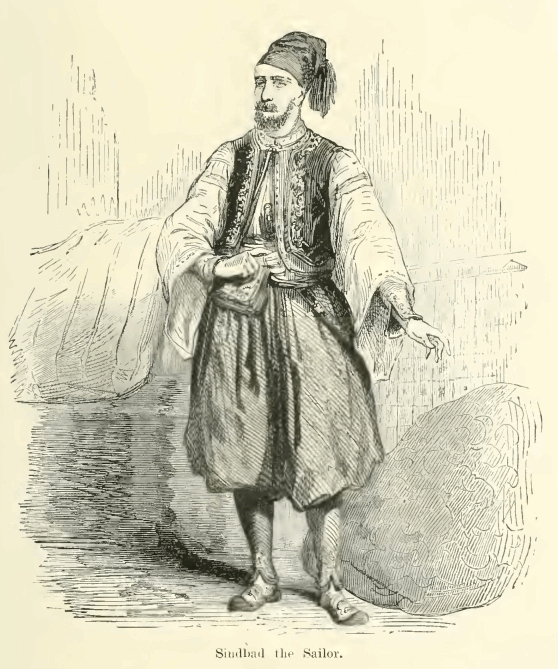
\includegraphics[width=\textwidth]{20093m.jpg}
\end{figure}

“But such services as these might involve him with the authorities of
the country in which he practices this kind of philanthropy,” said
Franz.

“And what cares he for that,” replied Gaetano with a laugh, “or any
authorities? He smiles at them. Let them try to pursue him! Why, in the
first place, his yacht is not a ship, but a bird, and he would beat any
frigate three knots in every nine; and if he were to throw himself on
the coast, why, is he not certain of finding friends everywhere?”

It was perfectly clear that the Signor Sinbad, Franz’s host, had the
honor of being on excellent terms with the smugglers and bandits along
the whole coast of the Mediterranean, and so enjoyed exceptional
privileges. As to Franz, he had no longer any inducement to remain at
Monte Cristo. He had lost all hope of detecting the secret of the
grotto; he consequently despatched his breakfast, and, his boat being
ready, he hastened on board, and they were soon under way. At the
moment the boat began her course they lost sight of the yacht, as it
disappeared in the gulf of Porto-Vecchio. With it was effaced the last
trace of the preceding night; and then supper, Sinbad, hashish,
statues,—all became a dream for Franz.

The boat sailed on all day and all night, and next morning, when the
sun rose, they had lost sight of Monte Cristo.

When Franz had once again set foot on shore, he forgot, for the moment
at least, the events which had just passed, while he finished his
affairs of pleasure at Florence, and then thought of nothing but how he
should rejoin his companion, who was awaiting him at Rome.

He set out, and on the Saturday evening reached the Place de la Douane
by the mail-coach. An apartment, as we have said, had been retained
beforehand, and thus he had but to go to Signor Pastrini’s hotel. But
this was not so easy a matter, for the streets were thronged with
people, and Rome was already a prey to that low and feverish murmur
which precedes all great events; and at Rome there are four great
events in every year,—the Carnival, Holy Week, Corpus Christi, and the
Feast of St. Peter.

All the rest of the year the city is in that state of dull apathy,
between life and death, which renders it similar to a kind of station
between this world and the next—a sublime spot, a resting-place full of
poetry and character, and at which Franz had already halted five or six
times, and at each time found it more marvellous and striking.

At last he made his way through the mob, which was continually
increasing and getting more and more turbulent, and reached the hotel.
On his first inquiry he was told, with the impertinence peculiar to
hired hackney-coachmen and innkeepers with their houses full, that
there was no room for him at the Hôtel de Londres. Then he sent his
card to Signor Pastrini, and asked for Albert de Morcerf. This plan
succeeded; and Signor Pastrini himself ran to him, excusing himself for
having made his excellency wait, scolding the waiters, taking the
candlestick from the porter, who was ready to pounce on the traveller
and was about to lead him to Albert, when Morcerf himself appeared.

The apartment consisted of two small rooms and a parlor. The two rooms
looked on to the street—a fact which Signor Pastrini commented upon as
an inappreciable advantage. The rest of the floor was hired by a very
rich gentleman who was supposed to be a Sicilian or Maltese; but the
host was unable to decide to which of the two nations the traveller
belonged.

“Very good, signor Pastrini,” said Franz; “but we must have some supper
instantly, and a carriage for tomorrow and the following days.”

“As to supper,” replied the landlord, “you shall be served immediately;
but as for the carriage——”

“What as to the carriage?” exclaimed Albert. “Come, come, Signor
Pastrini, no joking; we must have a carriage.”

“Sir,” replied the host, “we will do all in our power to procure you
one—this is all I can say.”

“And when shall we know?” inquired Franz.

“Tomorrow morning,” answered the innkeeper.

“Oh, the deuce! then we shall pay the more, that’s all, I see plainly
enough. At Drake’s or Aaron’s one pays twenty-five lire for common
days, and thirty or thirty-five lire a day more for Sundays and feast
days; add five lire a day more for extras, that will make forty, and
there’s an end of it.”

“I am afraid if we offer them double that we shall not procure a
carriage.”

“Then they must put horses to mine. It is a little worse for the
journey, but that’s no matter.”

“There are no horses.”

Albert looked at Franz like a man who hears a reply he does not
understand.

“Do you understand that, my dear Franz—no horses?” he said, “but can’t
we have post-horses?”

“They have been all hired this fortnight, and there are none left but
those absolutely requisite for posting.”

“What are we to say to this?” asked Franz.

“I say, that when a thing completely surpasses my comprehension, I am
accustomed not to dwell on that thing, but to pass to another. Is
supper ready, Signor Pastrini?”

“Yes, your excellency.”

“Well, then, let us sup.”

“But the carriage and horses?” said Franz.

“Be easy, my dear boy; they will come in due season; it is only a
question of how much shall be charged for them.” Morcerf then, with
that delighted philosophy which believes that nothing is impossible to
a full purse or well-lined pocketbook, supped, went to bed, slept
soundly, and dreamed he was racing all over Rome at Carnival time in a
coach with six horses.
